\documentclass[12pt,BSc,wordcount]{muthesis}
% The regulations say that 12pt should be used
% Change the MSc option to MPhil, MRes or PhD if appropriate
% Add 'anon' to the above options to replace your name with your student ID
\usepackage[left=2.15cm, right=2.15cm]{geometry}
\usepackage{verbatim}
\usepackage{graphicx}
\usepackage{tabularray}
\usepackage{url} % typeset URL's reasonably
\usepackage{listings}
\usepackage{tabularx}
\usepackage{amsmath,amssymb,amsthm}
\usepackage{thmtools}
\usepackage{hyperref}
\usepackage{pslatex} % Use Postscript fonts

% Uncomment the next line if you want subsubsections to be numbered
%\setcounter{secnumdepth}{3}
% Uncomment the next line if you want subsubsections to be appear in
% the table of contents
%\setcounter{tocdepth}{3}

% Uncomment the following lines if you want to include the date as a
% header in draft versions
%\usepackage{fancyhdr}
%\pagestyle{fancy}
%\lhead{}  % left head
%\chead{Draft: \today} % centre head
%\lfoot{}
%\cfoot{\thepage}
%\rfoot{}

\begin{document}
% Uncomment the following lines to leave out list of figures, tables
% and copyright until final printing
%\figurespagefalse
%\tablespagefalse
%\copyrightfalse

\title{OpenFitCompanion: a better fitness companion using trackers and AI}
\author{Egor Chernyshev}
\stuid{10660842}
\principaladviser{Lukas Hughes-Noehrer}

\beforeabstract

\prefacesection{Abstract}
%\abstracttitle
% Single spacing can be turned on for the abstract
%
{\singlespacing
Smart health-tracking devices and apps that leverage them have gained popularity as people become more health-conscious. However, due to the exclusiveness of many brands, the data is dispersed and not utilised effectively for guidance towards a healthier life. Many commercial apps try to tackle this problem, but most are inadequate in some criteria, such as transparency or cost. Profit incentives prevent users from receiving the best experience. The report presents OpenFitCompanion, an open-source, self-deployable, cross-platform application, designed as an event-driven composition of serverless microservices, that integrates data from fitness trackers to create helpful and highly personalised insights using a mixture of algorithms and LLMs.  Evaluating the final artefact for various criteria: cost, security and more, has shown that the application is a strong competitor to free apps on the market, but failing to present a better utility to cost ratio against paid apps. Nevertheless, it provides a strong foundation on which further improvements and optimisations can be applied, hopefully advancing the domain of fitness tracking apps towards more open and decentralised architectures.

Enabled by the core application, a research question: "Are examined devices different?" was investigated using two months of personal fitness data. Framing  the problem as an equivalence test and performing t-tests displayed evidence for significant difference in measurement of activity seconds at different intensities. However, the implications are akin to call for a further, more rigorous study,  as user errors and low sample size could have had an impact on the results. We believe that the application should help to facilitate such studies.
}



\afterabstract

\prefacesection{Acknowledgements}
I would like to thank my supervisor Lukas Hughes-Noehrer from the University of Manchester and the 
wearables research team at Manchester Royal Infirmary. I would also like to thanks my friends and family
for supporting me through my 3rd year of studies. 

\afterpreface

\prefacesection{Abbreviations \& Acrnonyms}
\begin{itemize}
  \item AWS: Amazon Web Services
  \item AI: Artificial Intelligence
  \item LLM: Large Language Model
  \item API: Application Programming Interface
  \item MET: Metabolic Equivalent of Task
  \item UI: User Interface
  \item RAG: Retrieval Augmented Generation
  \item IAM: AWS Identity and Access Management
  \item SNS: Simple Notification Service
  \item DLQ: Dead-Letter-Queue
  \item PWA: Progressive Web App
  \item VAPID: Voluntary Application Server Identification
  \item XSS: Cross Site Scripting
  \item CSP: Content-security policy
\end{itemize}
% These include the actual text


\chapter{Introduction}
\label{cha:intro}

\section{Motivation}
\par
In collaboration with NHS Manchester Royal Infirmary, I have received smart wearable devices - Withings Watch,
and later Oura ring. It was during a time when I wanted to improve my fitness, and so I had an initial idea of an
application that would act as a companion in a fitness journey. Such as reminding about daily activity, highlighting progress made and
possibly autonomously making suggestions from gathered wearable data. Researching existing product offerings, none of them 
did everything I envisioned, or they had major drawbacks such as cost.
\par One major point of contention with current wearables data tracking apps is that they are all closed-source offerings
 from for-profit corporations such as Google, Apple etc.
 Those apps are often predatory, following the well-known pattern in tech products, offering
 services for free to hook the user, and then pay-walling existing features to start getting profit margins once the user base has sufficiently grown. 
 One stark example is - MyFittnessPal, locking the previously free beloved feature of 
 calorie counting behind a premium \cite{myfitnesspalPaywall} as well as having a data breach that leaked sensitive health data of 150 million users \cite{myFitnessPalDataBreach}.
 My colleague who also worked with a Withings watch had their data deleted from their Withings app, probably caused by inactivity, as they stopped using the device after collecting enough data for their project. 
 This highlights the need to minimise reliance on such systems. I think that a community-driven open-source solution is a better approach. 
 It enables better security through faster vulnerability patching, as well as making it impossible to introduce predatory practices \cite{openSourcePredatoryProtect} By self-deploying the application, users would only pay for what they use on a pay-as-you-go basis. 
\par
In the wider context, this topic is important because fitness is closely linked with a person's overall health, being a risk factor in developing depression, heart diseases and more \cite{nhsObesity}. 
Fitness levels have been on the decline in both the UK and the rest of the world.
For example, as of Nov. 2021, 63.5\% of adults in England are either obese or overweight \cite{ukObesity2023Survey}. 
In Nov. 2022, It was estimated that obesity costs NHS £6 billion annually \cite{nhsObesityCost}.
Therefore, there is a large interest from institutions such as NHS to use technology to help combat this problem.

\par Smart Wearable devices can continuously and autonomously collect metrics about heart, activity, 
sleep and more. That data can then be used to autonomously derive insights, such as providing weekly exercise consistency. 
This eliminates the monotony of manual information tracking, as users don't have to do anything other than wear the devices,
 allowing them to focus on what matters. By using multiple devices, we can correct for inaccuracies of a single device. 
 The focus of this project is on wearable devices, however there is also potential to get further fitness data, and thus better quality insights, from stationary smart devices such as smart scales.

\par AI can be used to extract much more complex insights than any hand-crafted methods. With the recent advancements,
 namely LLMs such as GPT4, the quality of inferences and ease of use have never been better than before. In particular,
 those models are good at utilizing large amounts of context information to influence the result, this can be wearables data in this case. Also, those models are pre-trained, so we avoid issues of machine learning projects: creating a dataset, ensuring no bias, tweaking hyperparameters, training for large epoch counts to get adequate accuracy, etc.  As such, there is a large opportunity to explore how those models can help with the problem at hand. This is something that a few product offerings 
 have implemented recently, however, their pricing is astronomical and is not easily accessible to lower-income individuals. More on this in [].


On a personal note, what I found to be the hardest with fitness is staying consistent. It is especially tough because you don't 
see results immediately and it feels that you are not progressing. It is also very tedious to manually track fitness-related metrics.
Lastly, there might not be somebody who gives you encouragement or holds you accountable. I wanted to address all of those factors in my application, hoping it would help somebody out there as it helped me.
\section{Aims}
On a high-level, those are the aims I wanted my application to fullfil.
\begin{center}
    \begin{tabularx}{1\textwidth} {| >{\centering\arraybackslash}X 
        | >{\centering\arraybackslash}X 
        |}
    \hline
    Aim & Criteria for success  \\ 
    \hline
     1: Autonomously sync in real-time with several fitness devices, storing data in our database and producing single unified measurement as well & Concrete implementation, with example shown, to sync with Withings And Oura products, creating unified measurement by averaging.  Infrastructure to allow easy implementation of sync with other providers\\ 
    \hline
     2: Report to the user about their progress via notification, providing useful metrics and insights & Implementation to send push notification to the user's phone, then providing metrics on a separate page. Such as if the user fulfilled expected daily activity levels. \\ 
    \hline
     3: Integrate AI to analyse the data and provide accurate and effective feedback about the user's health and well-being & Concrete implementation using GPT4, provides feedback for each day, week and month. Feedback should be factual, mention specific metrics/measurements, and include positive areas and areas that the user can improve on.\\
    \hline
     4: Nudge the user to participate in physical activities by recommending the best activities/exercises depending on a variety of customizable parameters and data available &  Implementation to send push-notifications throughout times of day, linking to AI planned activity plan for that time. Activities should have descriptions and videos on how to perform them. Activities should be well-suited for the user's preferences and the data collected.\\
    \hline
     5: Minimise the cost of running the service & Compare the cost of operating our service with the costs of competing similar systems. They should provide similar functionality in order for the comparison to be fair. \\
    \hline
     6: Service should be secure. Preventing unauthorized access to data or functionality & Data should only be accessible by the sole authorized user - the Owner. Utilize automatic security testing tools as well as manual review to demonstrate compliance.\\
    \hline
     7: Using the data gathered by the service, perform data analysis to compare measurement differences between devices. &  Comprehensive data analysis is performed, with evaluation of results as well as limitations of the analysis.\\
     \hline
     8: The service shall match the state-of-the-art commercial solutions in terms of performance, UI/UX and ease-of-use & Compare performance, UI and ease-of-use metrics/quality with state-of-the-art standard or products  \\
     \hline
    \end{tabularx}
\end{center}
\section{Description}
Putting aims of the core application into short text: OpenFitCompanion is an open-source health data aggregator similar to commercial products like MyFitnessPal or Apple Fitness+ but prioritising: transparency, cross-platform, self-deployed infrastructure, data ownership and low cost. Aiming to provide better insights by using cutting edge generative AI technologies, as well as automating health data administrative tasks, so that users can focus on the meaningful actions that improve their life.
\section{Report Structure}
\subsection{Background}
The chapter will introduce concepts, provide an overview of devices used and competing software products + their problems. Note that concepts and components will be introduced in the general scenario, their applicability, configurations and justification of choice is made in the core design section \ref{cha:core_system_design}
\subsection{Core design}
This chapter will walk-though the process of creating the core application - OpenFitCompanion. Going from requirements to full design, heavily supported by diagrams.
\subsection{Comparing devices}
This chapter walks through a supplementary project task of comparing data between devices used.
\subsection{Evaluation}
There is an evaluation for all of the aims, discussing whether criteria for success were met.
\begin{itemize}
    \item 1, 2: Functionality examples will be provided as well as pointing out some problems/limitations: \ref{}
    \item 3, 4: AI response quality will be examined, with examples of responses provided. 
    \item 5: Cost analysis will be performed, calculating monthly cost of running the service from my actual personal use. This will be compared with the cost of competing products.
    \item 6: Security analysis, using automatic web vulnerability scanners, as well as manual review of IAM roles for adherence to least privilege principle
    \item 7: Evaluation of data analysis results will be performed, stating significance of findings and limitations.
    \item 8: Front-end's performance, UI and system's set-up as a new user will be evaluated discussed
\end{itemize}
\subsection{Conclusions}
This chapter concludes the report, providing ideas for further work as well as my personal reflection on the project





\chapter{Background}
\label{cha:background}
\section{Literature review}
\subsection{Wearable trackers}
Consumer-based wearable activity trackers are now readily available and can provide individuals with the ability to objectively monitor their physical activity levels. In addition, when combined with the use of smartphone and computer apps, they may assist users through a range of motivational and tracking tools to better manage their personal health \cite{trackersBenefitGeneral}
There is plenty of research to suggest that using wearable activity trackers helps people become more physically active. A large systematic review has shown that, over a number of studies, there is significant increase in daily step count, moderate and vigorous activity as a result of using wearables \cite{trackersBenefitGeneral}. In particular, people with chronic illnesses experienced decreased systolic blood pressure, waist circumference, etc \cite {Franssen2020}; monitoring such patients using wearables after hospitalizations could help detect complications and prevent rehospitalization \cite{hospi}. People of older age can also benefit greatly, showing moderate increase in physical activity and mobility \cite{SOliveira1188}; there is indication of good acceptability of such devices among older adults \cite {Franssen2020}. Attractiveness, gamification, readability, feedback is what drives the health benefits such as commitment to daily physical activity \cite{NELSON2016364}. Wearables are not a magic bullet solution to fitness problem. Some studies that spanned larger periods of time have observed decrease in physical activity after an initial positive effect \cite{Finkelstein2016}, or in other words, use of wearable devices is not directly effective at modifying habitual behavior \cite{LI2021104487}. A number of examined devices did not report sensor accuracy output validity at all, allowing for overestimation or underestimation of metrics \cite{Lee2014ActivityTA}
\subsection{Nudging}
A nudge is “any aspect of the choice architecture that alters people's behavior in a predictable way without forbidding any options or significantly changing their economic incentives” \cite{nudgeDef} An example would be providing information, implementing default choices etc. Nudges are categorised into Type 1 and Type 2. Type 1 nudge typically relies on unconscious thought and a more simple in nature, for example, rearranging  the presentations of consumer items in food isles to high-light options that would have ordinarily been ignored \cite{NudgeCritical}. On the other hand, Type 2 nudge relies on conscious thought, those are more complicated and more costly, for example, long-term educational campaigns promoting exercise present the benefits of regular exercise, as well as the harmful effects of continuing to be sedentary. \cite{NudgeCritical}.  In the area of fitness, nudging has shown to increase physical activity and reduce sedentary behaviour,for example, placing banners that encourage using the stairs shown positive effects and an increase in stair use \cite{FORBERGER2022106922, Forberger2019}. Nudging has lower cost of intervention than something like an educational campaign, while still being effective \cite{nudgeCost}. Although nudging has been shown to provide decently sizable impact, there are doubts about whether it is enough to tackle problems such as fitness on national (UK) level , raising concern that is may just be a "smokescreen" for inaction at tackling the root causes  \cite{Raynerd2177}
\section{Similar Systems}
\label{section:similarSystems}
\subsection{Google Fit}
\subsection{Apple Health}
\subsection{Other}
\section{Devices Used}
\subsection{Withings}
\subsection{Oura}
\section{Cloud Infrastructure}
Cloud computing is a model for enabling convenient, on-demand network access to a shared pool of configurable computing
resources (e.g., networks, servers, storage, applications, and services) that can be rapidly provisioned and released with minimal
management effort or service provider interaction. \cite {cloudDef}
Using cloud for the software service infrastructure has the benefit of off-loading complexity to cloud providers instead of handling it yourself. The services they provided are characterized as follows \cite{cloudServicesCategories}: 
\begin{itemize}
    \item 
\end{itemize}
\subsection{Software Requirements}
There 3 different types of requirements relevant to the domain of software: user requirement describing goal that specific class of user must be able to perform, functional requirement describing what developers must implement to enable users to accomplish tasks (user requirements), Business requirements describing high-level business objective of the organization that builds the system and optionally non-functional requirements, describing more qualitative features the system should have \cite{wiegers2013software}. Business requirements are not relevant to this project, as the main idea is open-source and self-deployment, meaning the project won't bring any commercial value to the creators. 
In general, requirements engineering has shown to improve design performance by facilitating sensemaking (learning about the project context)
User requirements can be understood by non-technical person. They can be represented using user stories, use cases and event-response tables. User story represent requirements using a simple textual template: "As a <role> I can <capability>, so that <receive benefit>" \cite{userStories}. Acceptance criteria may also be attached to a user story, containing details under which testable conditions the story can be considered completed \cite{Kannan2019User}. One of the popular templates for an acceptance criteria is: " Given <conditions>, When <action taken>, Then<outcome of action taken>". Although many practitioners testify that the technique is effective, improving productivity metrics within the team; however, it is only a perceived effectiveness that is not scientific \cite{userStories}.
Functional requirements are more technical, and are intended to be used as description of a system that engineers need to implement. \cite{wiegers2013software}. Although purely textual representations exist, more detailed representations that utilize diagrams are preferred. (System) Use Case Diagram is a UML diagram used to specify functionality offered by the system. \cite{malan2001functional}. Requirements with lots of conditionals can be represented as flow chart, or if the requirement is simple, it could be represented as a sentence in the style of user story. 


\subsection{Cloud Providers}
There are 3 major providers in this space: AWS, Azure and GCP. They fall into public cloud category, similar to utility services like Electricity, they are available for use to anyone, be it individual developer or a company. We are relying on third-parties to handle things such as legal compliance, disaster management etc. Providers outline their legal promises in the document called Service Level Agreement (SLA) \cite{cloudSLA}. Outlining major cloud provider's differences:
\begin{itemize}
    \item {he}
\end{itemize}

I chose AWS for this project for the following reasons:
\begin{itemize}
    \item{AWS has the best security system [cite], mainly due to IAM service, allowing for tight control of what a resource allowed to access in the infrastructure. }
    \item{if used under similar conditions, such as hosting the database in the same region in all comparisons, AWS has among the best quantative performance metrics, such as availability, latency etc \cite{CloudMetrics}  }
\end{itemize}
\subsection{Serverless}
\subsection{Security}
Software Security is important, especially in the context of this project that deals with sensitive health data. Generic web-accessible recommendations should apply to this project, such as encryption, xss, etc. However, deploying the application on the cloud presents new security related challenges, which a lot of companies suffer from [cite]. 
\section{LLMs}
"A large language model is the language model with massive
parameters that undergoes pretraining tasks (e.g., masked
language modeling and autoregressive prediction) to un-
derstand and process human language, by modeling the
contextualized text semantics and probabilities from large
amounts of text data " \cite{Yao2023ASO}
Unlike neural networks, the main way to improve response quality is to improve the prompt \cite{Liu2021PretrainPA}; "Prompt Engineering" is the technique for doing that, maximizing utility of LLMs in various tasks \cite{zhou2023large}
 In 2022, OpenAI made GPT3 available to the public, a product that surpassed Google in daily webpage visits. It revolutionized AI, in a way that a lay person could use it with some decent efficiency. The vital factor is it's ability to effectively utilize context window, a collection of prior information (such as prior messages sent in a chat) that is used to influence the next output. The workflow of using GPT3 as a software developer is as follows: Explicitly attach context messages together with a prompt. The complexity of managing contexts was upon your system that uses the OpenAI API. This recently changed with Assistants API. This feature allows creating of assistants, which can have threads that correspond to continuous chat with a user. Key factor is that the complexity of maintaining context is handled by OpenAI. Also it features OpenAI's own Retrieval Assisted Generation (RAG) solution named Knowledge Retrieval. RAG is a functionality that allows LLMs to access relevant external knowledge and use it for response generation. It is usually more prioritised that the ordinary context,significantly reducing the chances of hallucinations and improving output quality. [cite]

% On 4th March 2024, Shortly after finishing the project implementation, Anthropic announced Claude 3 Sonnet. It's benchmark scores are similar or better than gpt-4-1106-preview, it has bigger context window but costs 333\% less. This makes the reasoning behind the choice of gpt-4-1106-preview not valid at the moment of writing the report, however it was valid at the time of planning for AI functionality at the time of Dec 2023. 
\chapter{Core Systems Design}
\label{cha:core_system_design}
\section{Requirements Analysis}
\subsection{User Requirements}
The following user requirements for the system were gathered by inspecting similar systems, personal creativity and feedback from supervisor or wearables lab team. User stories were chosen for representation: \ref{table:userStories}.
\begin{center}
        \begin{longtblr}[
            caption={User Stories},
            label={table:userStories}
        ] {
            colspec = {|X|X|},
            rowhead = 1,
            hlines,
        }

        User Story & Acceptance Criteria  \\ 

        As a user I can view health data originating from Oura and Withings devices on a single central dashboard UI, so that I can quickly compare measurements between the devices and also manually examine my physical activity and sleep trends.
        & 
        Given that user is authenticated, when the user is on the dashboard page, the dashboard is displayed, containing a graph visualising last 7 days of data from both devices, with each line colored differently for each device; also buttons to switch which property, such as steps per day, should be displayed on the graph.
        \\ 

        As a user I can download all of my data as a csv file by pressing a button in the UI, so that I have my personal data conveniently in one file, in a widely supported format, which could be used for backing-up my data tp other storage solution, running data analysis etc.
        & 
        Given that user is authenticated, when the user presses 'Export CSV' button on the main page's UI, the csv file download starts, with that file containing all of the health measurements data persisted in the system's database at that time 
        \\ 

        As a user I can critically reflect on the passed day, with helpful insights and data presented on the UI; I also want to be reminded about this everyday at a certain configurable time; So that I can assess my progress towards my health goals, take pride in my accomplishments today and identify areas to improve on tomorrow.
        & 
        Given that user is authenticated, at a user configured time, the user is notified about daily report being available. On the daily report UI page, there is feedback highlighting areas of achievement and areas to improve on; as well as a graph visualising user's progress towards their weekly activity goals, as well as how well/poor the predicted daily activity norm was achieved
        \\

        As a user I can critically reflect on the passed week, with helpful insights and data presented on the UI; I also want to be reminded about this everyday at a certain configurable time; So that I can assess my consistency in physical activity or sleep, as well as compare this with the previous week.
        &
        Given that user is authenticated, when the user configured time is reached, the user is notified about weekly report being available. On the weekly report UI page, there are graphs visualising consistency in key metrics of MET minutes and sleep score; as well as numerical value quantifying the consistency, with a comparison to the 3 previous weeks. 
       \\

       As a user I want to receive activity reminders throughout the day at configurable times containing a list of curated exercises, with description and video example on how to perform them, that are well suited to my preferences and health data so far in the week; So that I am encouraged to fullfil my weekly activity goals; saving time by not having to create a good exercise regiment myself or saving money by not paying somebody else to do it.  
       &
       Given that the user is authenticated, when the user configured time is reached, the user is notified about daily exercise. On the exercises UI page, there is achieved to expected activity counter and curated list of exercises, which respect the following user configured preferences: athleticism level, MET weekly target, excluded activities, gym days and home equipment; as well as taking gathered health data into consideration.
       \\
       As a user I can submit free-form natural language questions and then receive natural language answers, which should be influenced as required by my health data and my profile; accessible though UI. So that I can have natural conversation about my health like I would with a real-life personal trainer, providing guidance and sense of not being alone.
       &
       Given that the user is authenticated, when the user visits the the AI Chat UI page there is a chat containing past user's requests and system's responses; there is an input box where the user can type a question using natural language. After submitting the question a reply is sent, which takes into account user's health data and their profile.

        \end{longtblr}
    \end{center}

\subsection{Functional Requirements}
The following functional requirements were derived so that user requirements could be fulfilled. System use case UML diagram, Flowchart and textual descriptions were used as representations.
\begin{itemize}
    \item Sync and view data diagram: \ref{fig:2}
    \item Export data diagram: \ref{fig:3}
    \item Daily \& Weekly Reports diagram: \ref{fig:4}
    \item AI Inference flowchart: \ref{fig:5}
    \item Activity Plan diagram: \ref{fig:6}
    \item Personalisation: User is able to configure their profile, which is saved in the database and used to customise modifiable parameters of the system. The profile has the following fields: 
    \begin{itemize}
        \item Height in Cm: Integer
        \item Weight in Kg: Integer
        \item MET Minutes weekly target: Integer
        \item Excluded Activity Keywords List of strings
        \item Athleticism: Enum [Beginner, Intermediate, Expert]
        \item Gym Days: List of Days of the week
        \item Home equipment: List of strings
        \item Report notification time: Time
        \item Daily Activity Reminder times: List of Times
    \end{itemize}
\end{itemize}
\begin{figure}
    \centering
    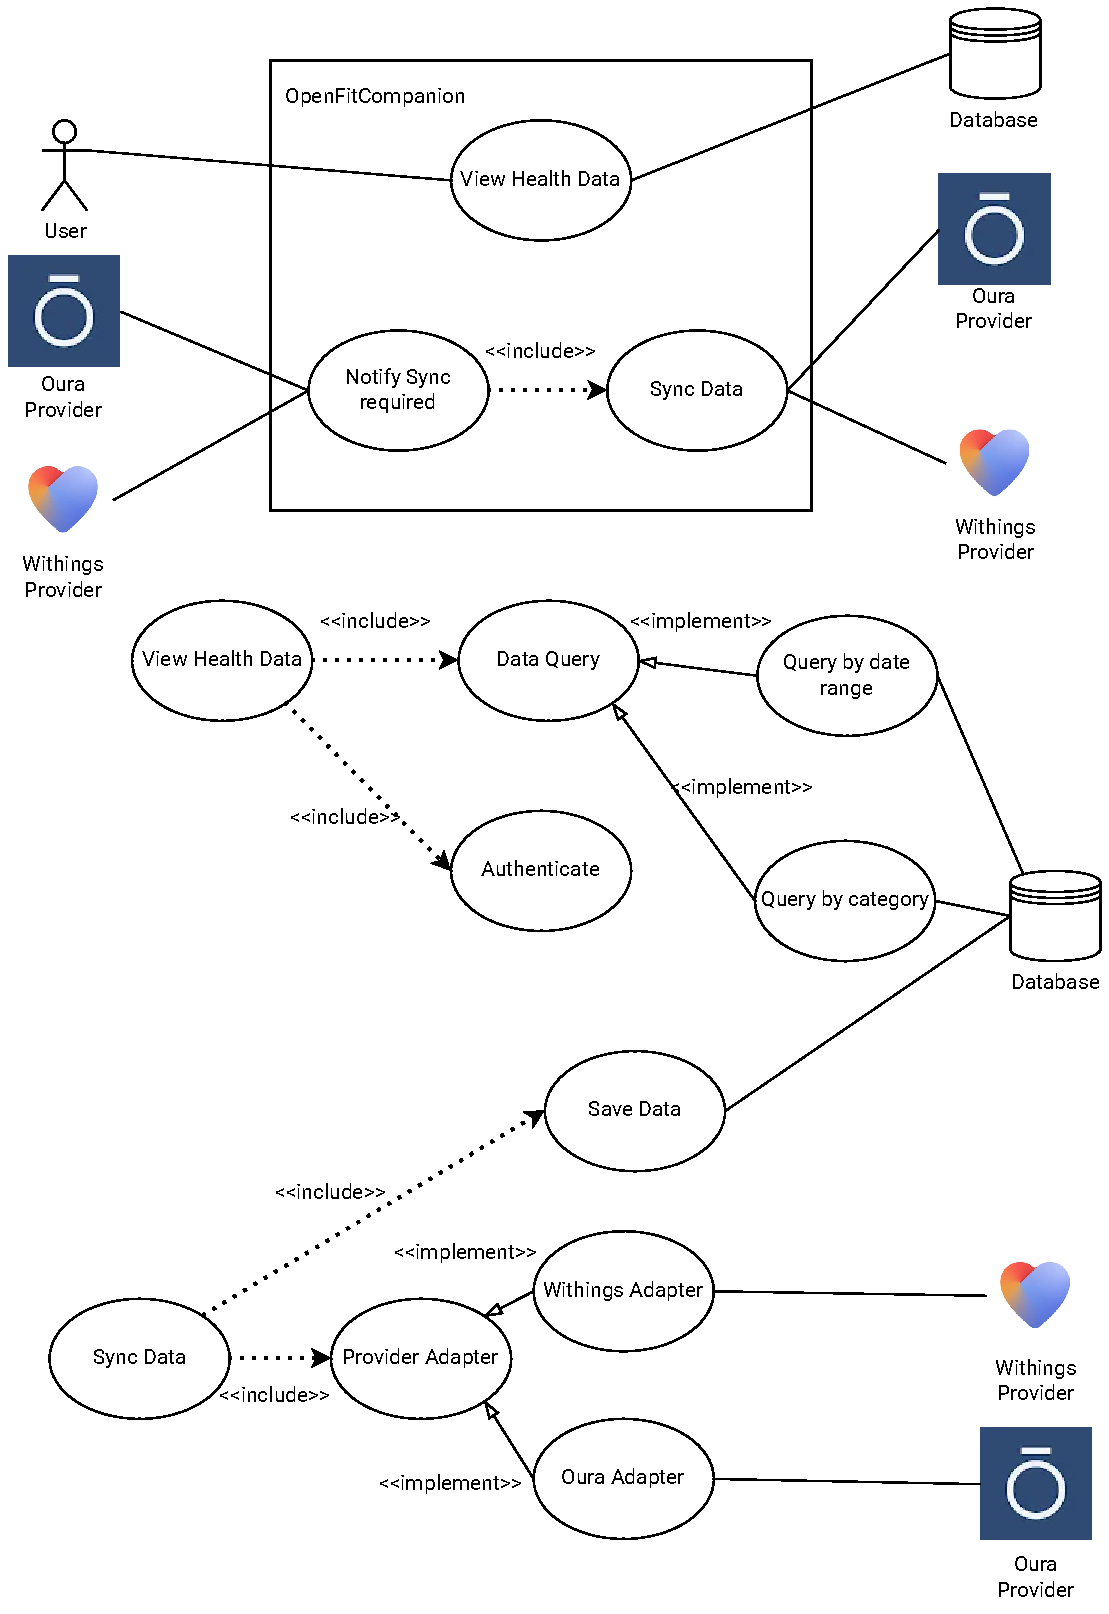
\includegraphics[width=\textwidth,height=\textheight,keepaspectratio]{../images/viewFunc.pdf}
    \caption{View data use case UML diagram}
    \label{fig:2}
\end{figure}
\begin{figure}
    \centering
    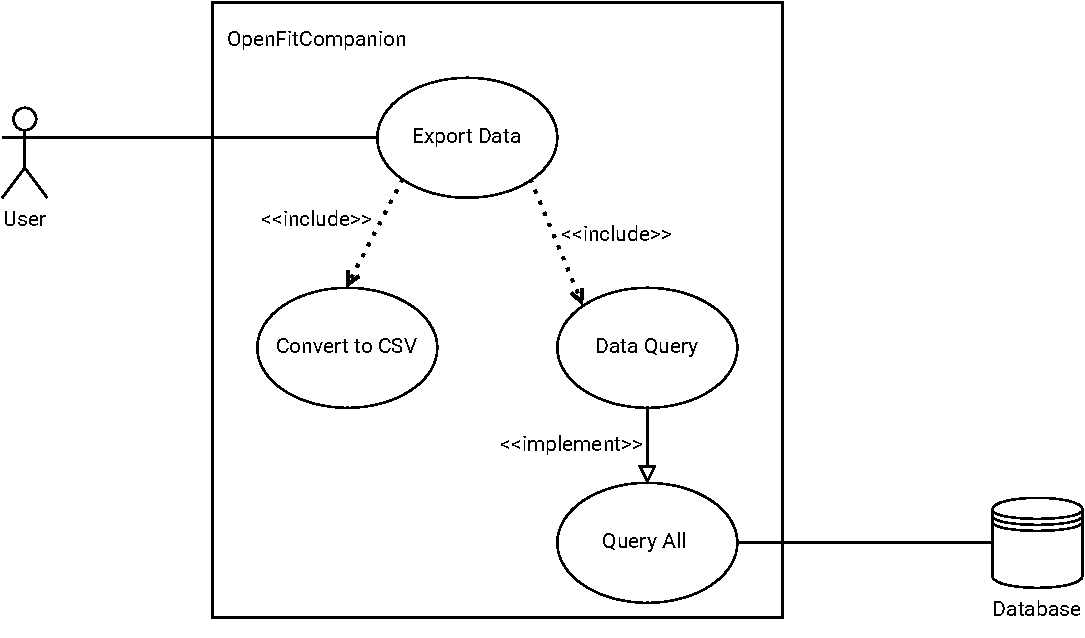
\includegraphics[width=\textwidth,height=\textheight,keepaspectratio]{../images/exportDataFunc.pdf}
    \caption{Export data use case UML diagram}
    \label{fig:3}
\end{figure}
\begin{figure}
    \centering
    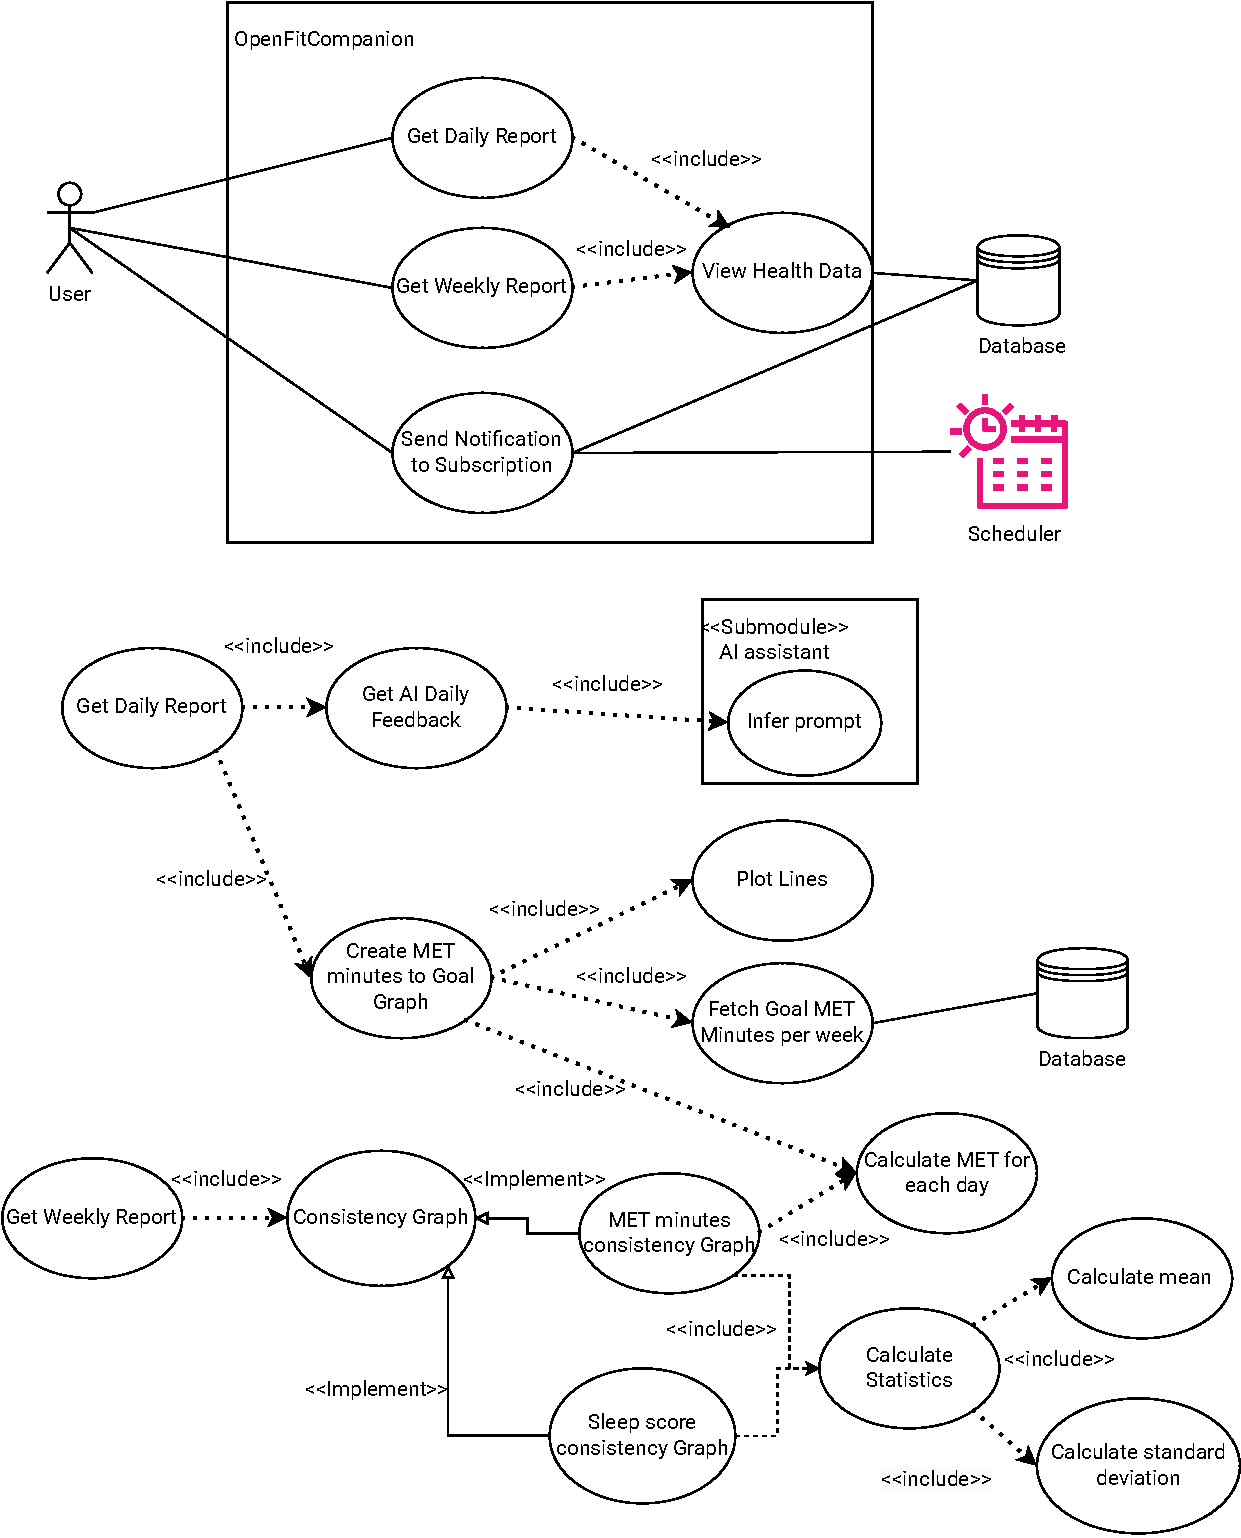
\includegraphics[width=\textwidth,height=\textheight,keepaspectratio]{../images/reports.pdf}
    \caption{Daily \& Weekly Reports use case UML diagram}
    \label{fig:4}
\end{figure}
\begin{figure}
    \centering
    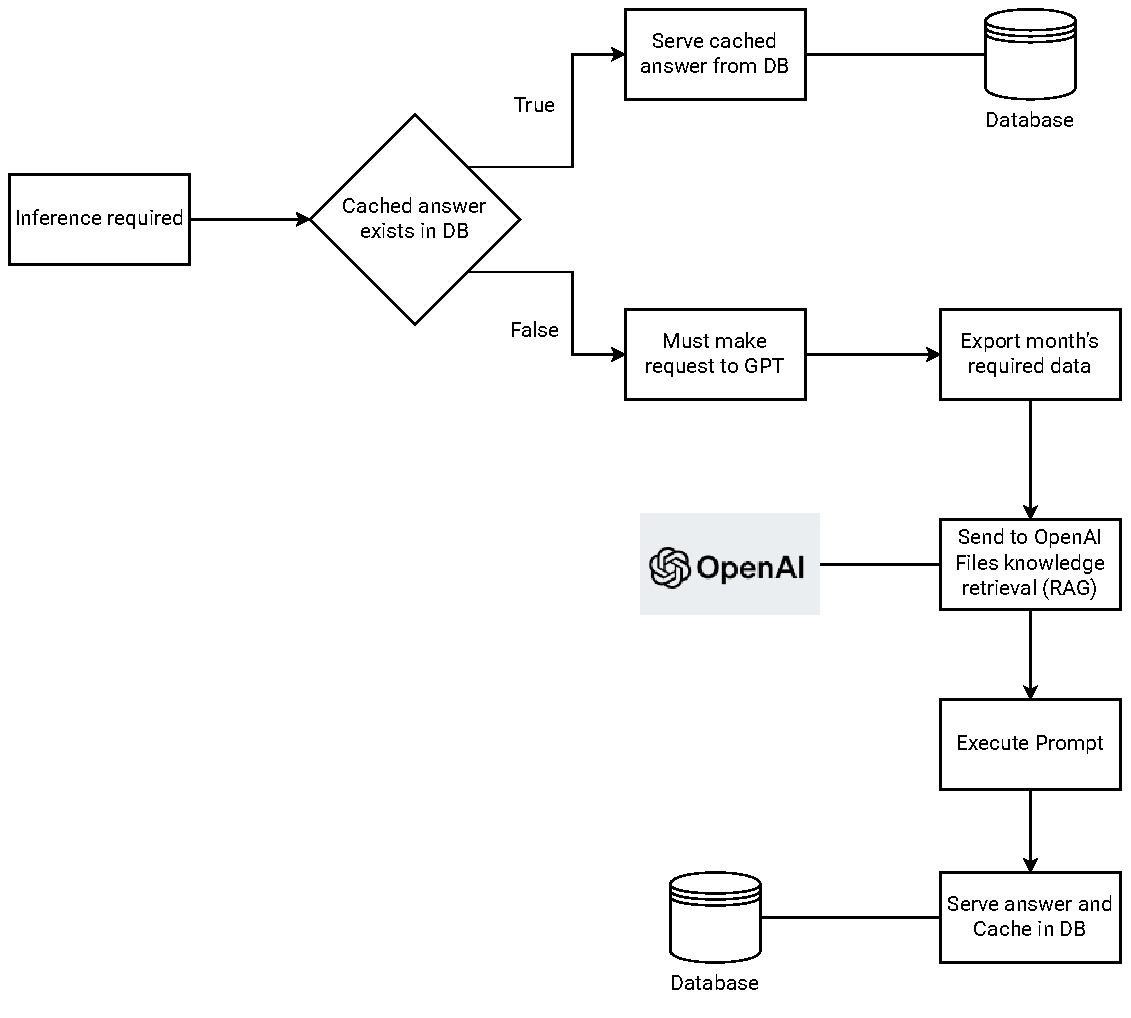
\includegraphics[width=\textwidth,height=\textheight,keepaspectratio]{../images/ai.pdf}
    \caption{AI Inference functionality Flow Chart}
    \label{fig:5}
\end{figure}


\begin{figure}
    \centering
    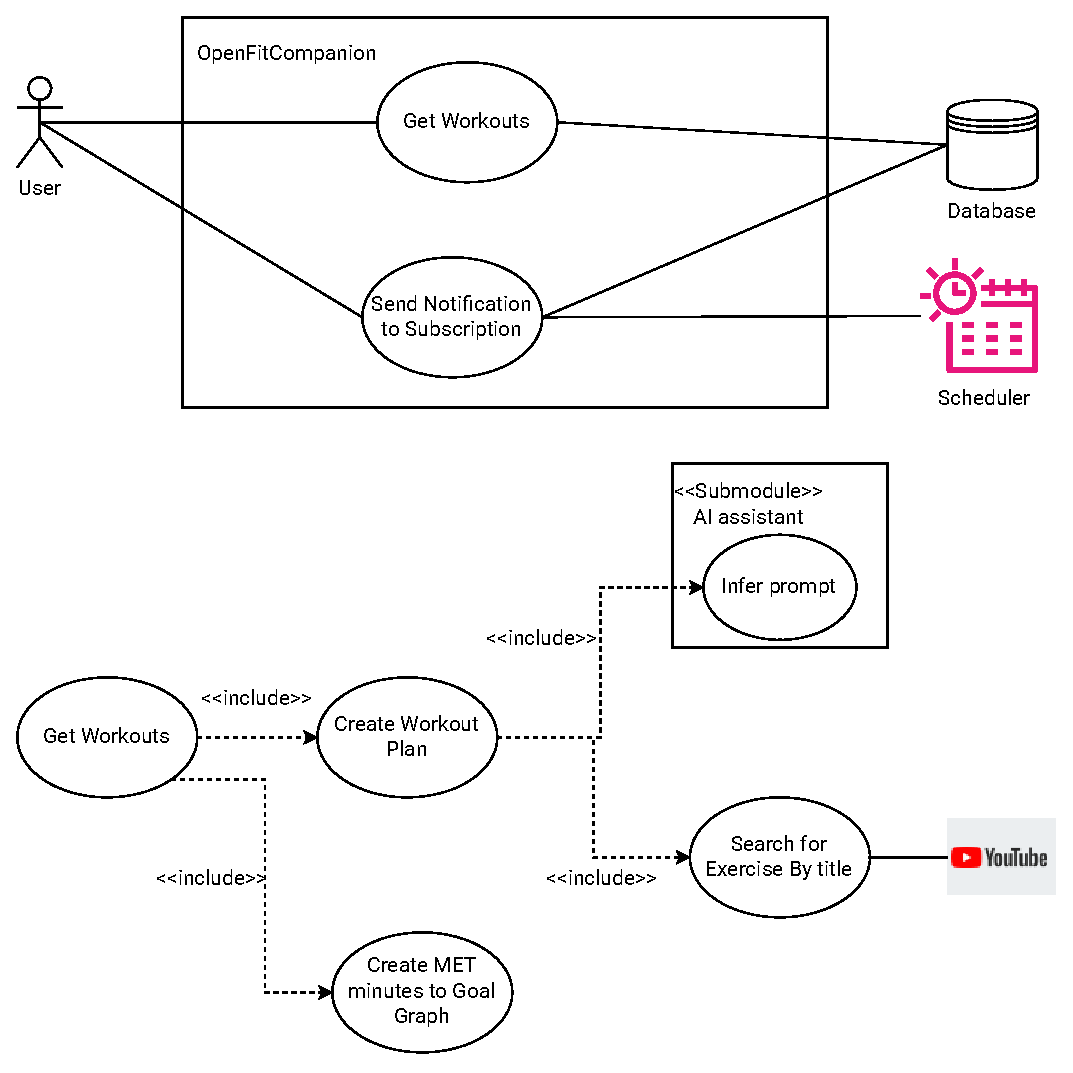
\includegraphics[width=\textwidth,height=\textheight,keepaspectratio]{../images/workouts.pdf}
    \caption{Activity plan use case UML diagram}
    \label{fig:6}
\end{figure}
\subsection{Non-Functional Requirements}
The following non-functional requirements for the system were gathered by inspecting general best practices and common sense. Represented as textual descriptions. 
\begin{itemize}
    \item Security: System must be secure and only allow access to the authenticated user. 
    \item Performance: UI must have low latency and feel snappy when used on a mobile network. 
    \item Usability: UI must be comfortably usable on mobile; openable as a native mobile app, supporting push notifications in the background (even if app is closed)
    \item Accessibility: UI must follow best practices supporting usage with assistive technologies such as screen readers, keyboard only etc
    \item Extensibility: The whole system should be easy to maintain and add new features; feature comprehensive logging and scale to add more providers
    \item Cost: Cost of running the service should be minimised while retaining required functionality.
\end{itemize}
\section{High-level overview}
\begin{figure}
    \centering
    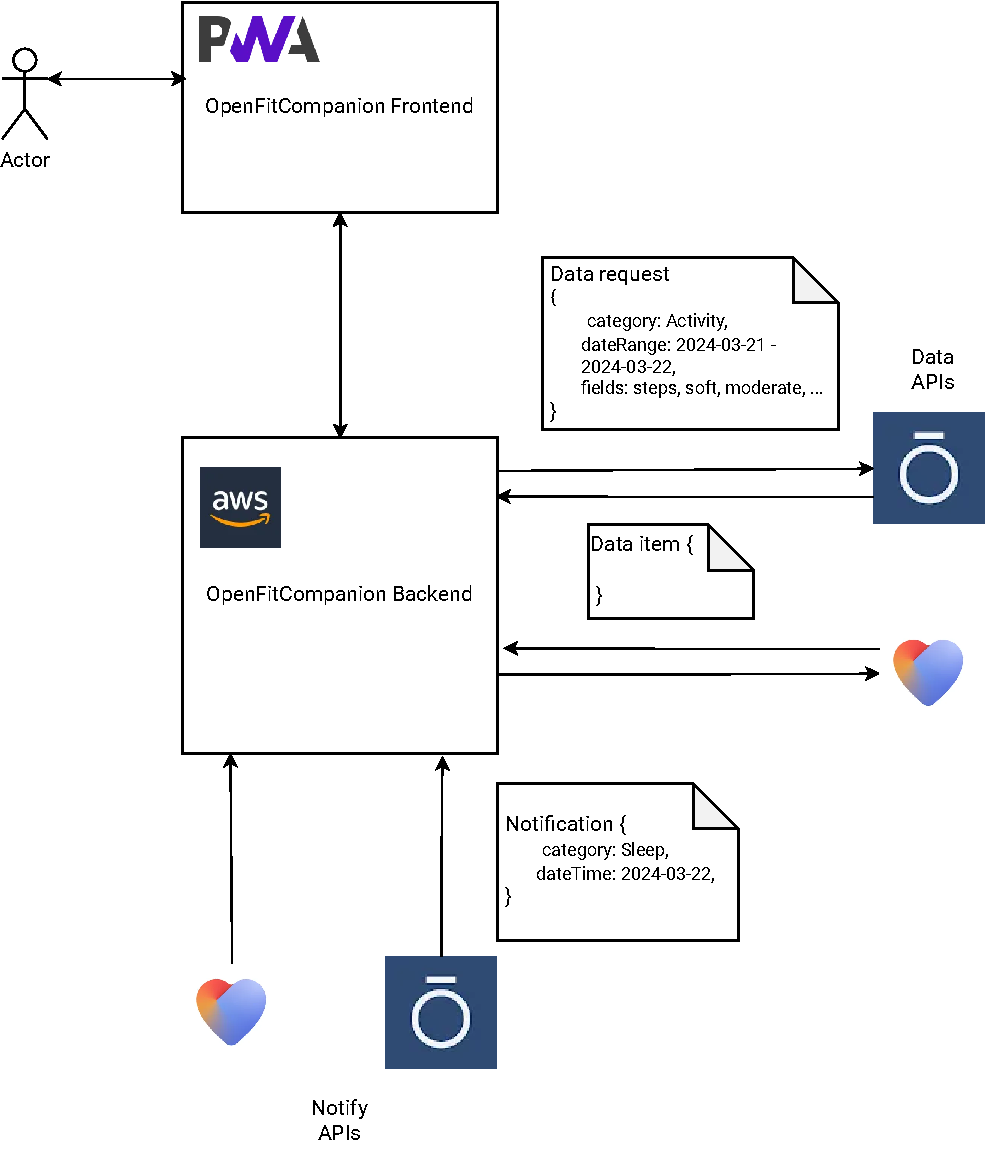
\includegraphics[width=\textwidth,height=\textheight,keepaspectratio]{../images/highLevel.pdf}
    \caption{High-Level architecture diagram}
    \label{fig:1}
\end{figure}
Overall, the architecture is considered event-driven. Computation only needs to happen in response to an external event. This is enabled by providers providing Webhook integrations. Essentially, the backend gets a notification from providers whenever there is new data available from them. The following is the diagram together with sample data exchanged: \ref{fig:1}

Cloud deployed backend service receives notifications from providers, containing information that allows atomic processing of that notification. It does not matter what other requests came before or if any are executing at the moment. 

In response to the notification, backend sends a request to Data APIs of providers, receiving an item(s) back and finally persisting it in a database for further purposes. 

Withings and Oura providers were integrated at the time of this report. However, the system can scale to many more providers. The only requirement for a provider is that they have Data API we can use. Even if a particular provider did not have a webhook (notification) service, we could re-sync with data APIs on regular schedule, like every 30 minutes. With the interval value being a trade-off between potentially more latency in syncing the data or wasted compute time when there are no updates. This would be quite costly if the system was publicly available service, as that scheduled request would be needed for each user. However, for our use case of self-deployed service, the cost would be negligible. However, there is still reliance on provider's API services to get the actual data from devices. System does not communicate with the smart devices directly via Bluetooth, there is an intermediate provider's system that data must be pass through. So, if a provider does not have such service, we can't integrate their devices into the system. However, all providers examined at least provided Google Fit integration, from which the data could be fetched instead. 

Ultimately, the data is transformed into useful information (insight) using using LLMs and classical algorithms. This is then presented to the user through the frontend. 
\begin{itemize}
    \item {Dashboard, contains a graph visualizing data from all devices, allowing for comparison and a brief overview of trends.}
    \item {Daily Report, containing a graph visualizing MET minutes completed this week and the goal MET minutes per week; Feedback on expected activity completion for that day and AI feedback for that day. Provides the user with information, allowing them to reflect on their day, seeing the progress towards fulfilling the weekly activity goal. A notification is sent to the user when such report is available. This constitutes Type 2 nudge, as it  engages user's conscious, reflective thinking to get them more motivated for physical activity tomorrow. However, there is also a component of Type 1 nudge with report notifications being opt-out rather than opt-in.}
    \item {Weekly Report, focusing more on consistency rather than absolute values and goal completions. Contains a graph visualizing deviation from the mean value of daily activity or sleep score. Same nudging as Daily Report.}
    \item {Activity plan, containing curated list of planned physical activities for the day, generated by AI. Also containing feedback about activity minutes done today. Similarly, it has type 1 nudging factor, being opt-out as well as Type 2 nudging, by notifying users at certain times when they should be doing exercises, and providing well-suited list of exercises, with description of benefits and video examples on how to perform them. This removes the need for user to plan their own workouts, removing decision paralysis. This imitates real-life coaching with a personal trainer, bringing benefits such as accountability and personalisation to users who may not be able to afford the real counterpart.}
\end{itemize}

\section{Back-end}
Because the system is event-driven, we can utilise serverless function as the main computing units in the backend; For AWS that is Lambda. Using Lambda is the most cost-effective option; it allows paying only for execution time down to milliseconds, free data out transfer to other AWS services. One disadvantage are cold starts, when a function is called for the first time in a while, it has increased latency due to some set-up, from my experiments it's around 400ms on average; and that happens for all Lambda functions, so if there is a chain of such functions called one after another, the latency will stack up and be quite noticeable. AWS provides the "Provisioned Concurrency", making sure that n functions are kept initialised and ready to respond at any time; however, it has a separate costing scheme similar to servers, whereby you pay by the second even if the function never called. As per project aims, minimising cost is more important so the latency is something that is just tolerated.

For persistance, DynamoDB is used. It is schemaless in the attributes, however the keys need to be set beforehand. Because the service is meant to be used by a single user who is the owner of the self-deployed infrastructure, there is no need to identify to which user the row of data belongs to. 
Some of the backend components are in \ref {}, as to not clutter the diagram and semantically they are more about interaction with the frontend.
\subsection{AWS services}
\subsection{Adapters}
\subsection{Unifying}
\section{Front-end}
\subsection{UI}
\subsection{Notifying}
\subsection{Reporting}

TODO: Do this chapter

\chapter{Comparing Devices}
To not repeat the names of the devices, the following shortening will be used: 
\begin{itemize}
    \item watch: Withings ScanWatch: \ref{section:WithingsWatch}
    \item ring: Oura ring Generation 2: \ref{section:OuraRing}
\end{itemize}
\section{Research Task}
The core application allows easy access to measurements from multiple devices in a CSV format. This enables researchers to analyse the data to answer research questions. As a supplementary project task, data analysis was performed to answer the following research question: "Do examined devices produce significantly different measurements for common fields?" Importantly, this is not the same as answering: "Are examined devices accurate?", as that would demand a much more rigorous study, requiring ground-truth measurements for every day, which are hard to acquire in practice, as those highly accurate devices are expensive, non-mobile, require technician, etc. Instead, the precision of the differences in device measurements is examined rather than the individual device's accuracy. 
\section{Data}
There are 60 days of personal data from both devices. Both devices were always worn at the same time, never one device but not the other. Both devices were configured properly - such as indicating the correct weight in both apps every week. That means that the data from devices is directly comparable. Lastly, only common measurements were used; the only non-common measurement was REM sleep duration, which the watch does not measure, so that field was deleted from the ring's rows for the analysis.
% TODO technologies in backend.
\section{Exploration}
Python with pandas, numpy and statsModels were used for analysis. To explore the dataset, a Bland-Altman plot was created on various common measurements. The difference in measurements for the same date is calculated by: $\text{ring[property]} - \text{watch[property]}$, meaning that negative values mean that the ring's measurement was lower than the watch's.
\begin{figure}
    
    \centering
    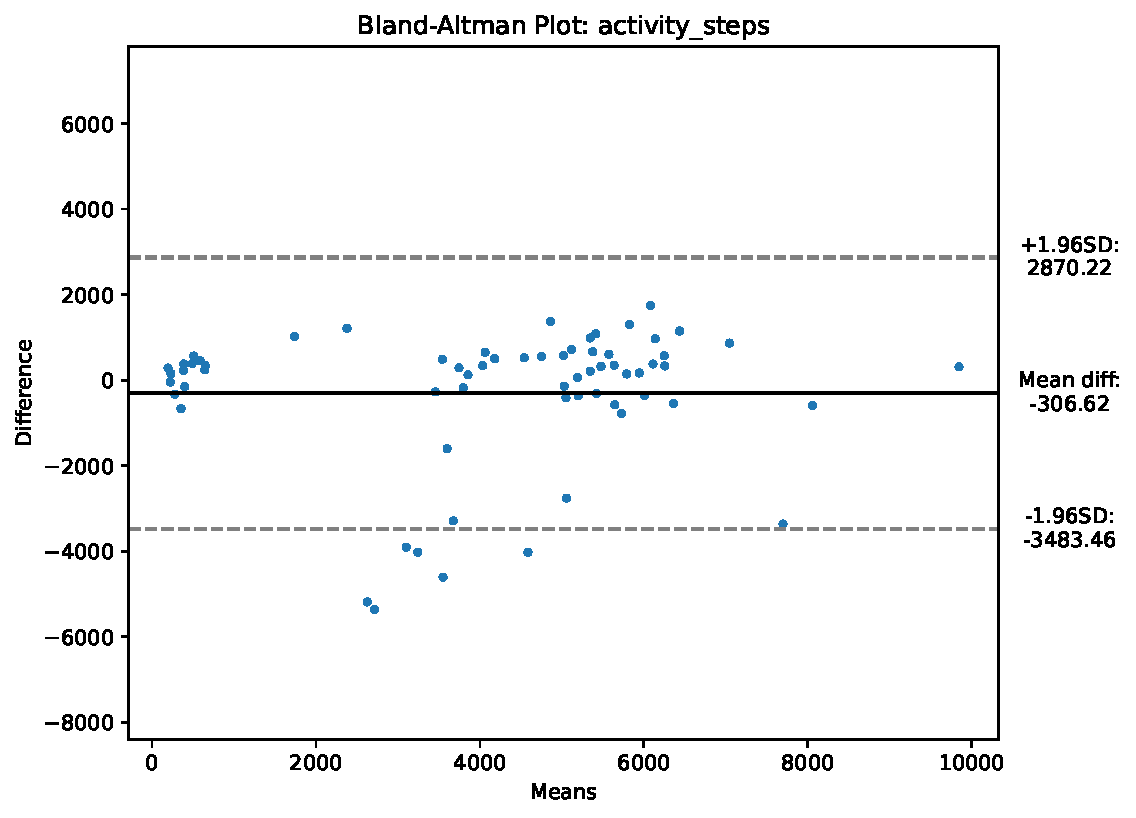
\includegraphics[width=\textwidth,keepaspectratio]{../images/bland_altman_steps.pdf}
    \caption{Bland-Altman Plot for Steps}
    \label{fig:blandAltmanSteps}
    
\end{figure}

For steps \ref{fig:blandAltmanSteps}, the average difference between devices is quite small, with the watch recording 306 more steps; for example, if the watch recorded the daily recommended number of steps - 10000, then the ring would have 9694 steps, which is only 3.06\% away from the goal. Overall, there is not a lot of variability in the differences, as points are mostly vertically clustered around the mean difference line. However, the mean difference is greatly affected by outliers, which are unlikely to occur naturally; more than a 4000 step count difference, which is more than two standard deviations away from the mean, does not make much sense and is most likely due to some error. 
\begin{figure}
    
    \centering
    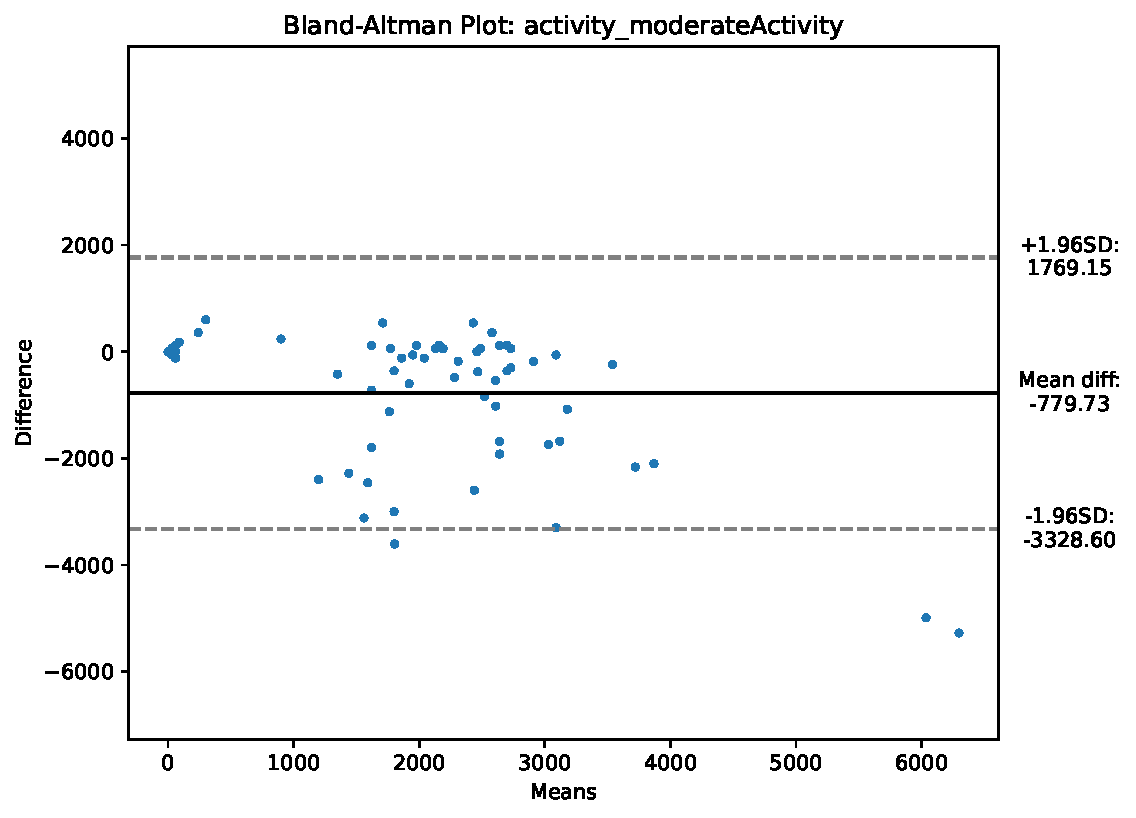
\includegraphics[width=\textwidth,keepaspectratio]{../images/bland_altman_moderateActivity.pdf}
    \caption{Bland-Altman Plot for Moderate Activity Seconds}
    \label{fig:blandAltmanSoftActivity}
    
\end{figure}

For moderate activity \ref{fig:blandAltmanSoftActivity}, the difference is more significant, with the watch on average recording 779 seconds (13 minutes) more. Although the difference might seem small, when considering how it translates into MET minutes, it has vital implications. For example, with a daily activity goal of 178 MET minutes, and using an MET factor of 3 for moderate activity, when the watch reached the goal, the ring only recorded 139 ($178 - 13 * 3$), which is 22\% away from reaching the goal; this adds up to missing 273 MET minutes in a week. Interpretation of this depends on which device is more accurate, if the watch is accurate then the ring underinflates, which is better than the other option that the ring is accurate and the watch overinflates, and of course, both could be slightly away from the true value. Assuming the ring is more accurate, users that use the watch might feel confident that they reached their activity goals to lose weight, when in fact they are missing a sizeable chunk of exercise, which could sabotage their confidence, as they might be losing less weight in reality than predicted. 

Although care has been taken to collect high-quality data, there might be user errors. Sometimes the watch could have lost contact with the skin due to a loose strap for comfortable wear, or some device turned off due to the charge running out. Also, development of the core product was still underway, so maybe some changes caused some notifications to be lost. To address outliers, z-scores are computed for each data point, and values for which: $-2 <= z <= 2$ are removed. The following are Bland-Altman plots with outliers removed for the examined properties: Steps \ref{fig:blandAltmanStepsNoOutliers} and Moderate Activity \ref{fig:blandAltmanModerateActivityNoOutliers}. The difference in step count went down to 114, which is a negligible difference, whereas the difference in the moderate activity remained relatively high at 10 minutes, suggesting some systematic difference between devices.

\begin{figure}
    
    \centering
    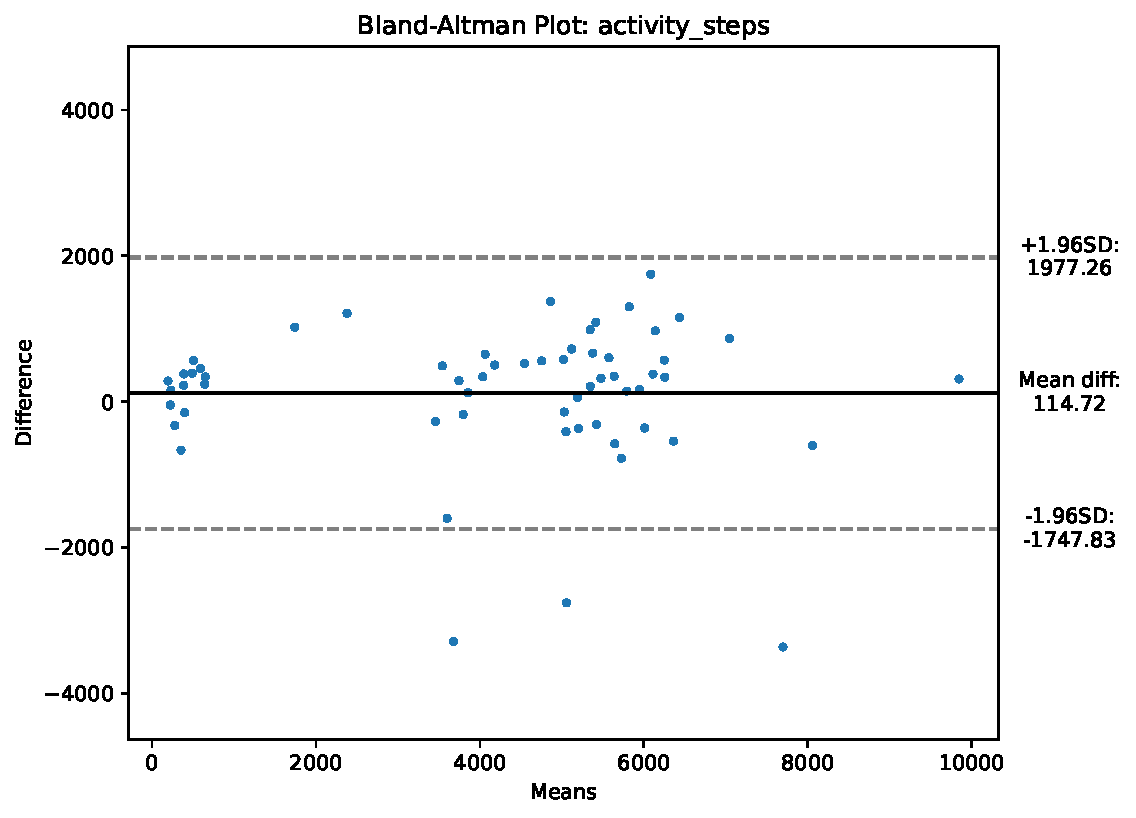
\includegraphics[width=\textwidth,keepaspectratio]{../images/bland_altman_steps_no_outliers.pdf}
    \caption{Bland-Altman Plot for Steps with previous outliers removed}
    \label{fig:blandAltmanStepsNoOutliers}
    
\end{figure}
\begin{figure}
    
    \centering
    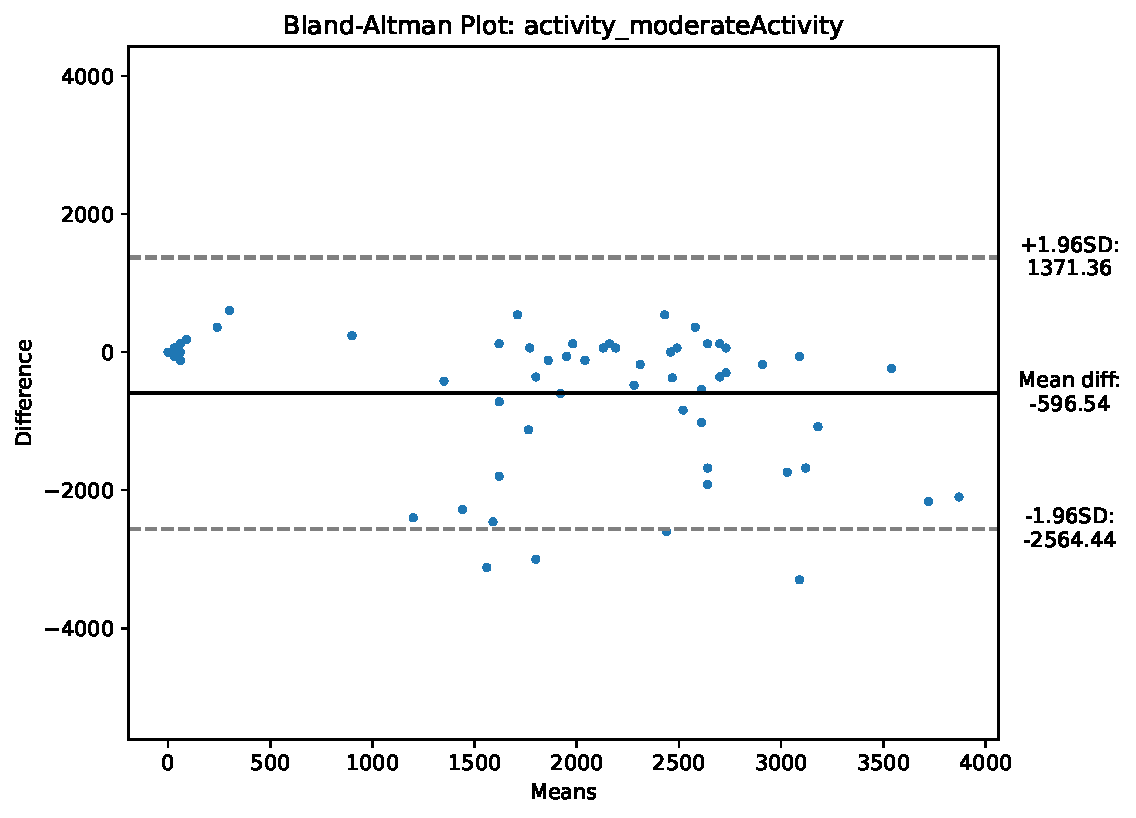
\includegraphics[width=\textwidth,keepaspectratio]{../images/bland_altman_moderateActivity_no_outliers.pdf}
    \caption{Bland-Altman Plot for Moderate Activity Seconds with previous outliers removed}
    \label{fig:blandAltmanModerateActivityNoOutliers}
    
\end{figure}
% TODO: background for bland altman, outlier detection - zscore, two one sided t-tests for equivalence bound, t-test.
\subsection{Average Percentage Difference}
The overall average difference between devices is 26.1\%, as calculated from the empirical data. Percentage differences per property: \ref{fig:empirical}. The calculation was performed as follows: 
\begin{itemize}
    \item Remove outliers using zscore.
    \item $a = \text{max}(a, 0.00001)$, $b = \text{max}(b, 0.00001)$ - prevent division by 0 errors.
    \item Calculate percentage difference: $\text{diffDate} = max(a,b) / min(a,b) \mod 1$. Modulo 1 extracts the fraction by which the larger value is bigger than the smaller one.
    \item Calculate average percentage difference: $\sum_{n=1}^{N} \text{diffDate}_n / N$.
\end{itemize}
\subsection{Statistical Testing \& Results}
Purely empirically, we could conclude that devices are different as we have a high number: 26.1\%. However, statistical significance at a certain confidence needs to be considered to make more formal conclusions. The following equivalence hypothesis testing problem was formulated for every measured property, such as steps: 

Let $\mu_1$ be the true mean of the watch's measurement of the inspected property, $\mu_2$ be the true mean of the ring's measurement of the inspected property
\begin{align*}
    H_0:\mu_1 = \mu_2 \\
    H_1: \mu_1 \neq \mu_2
\end{align*}
\begin{figure}
    
    \centering
    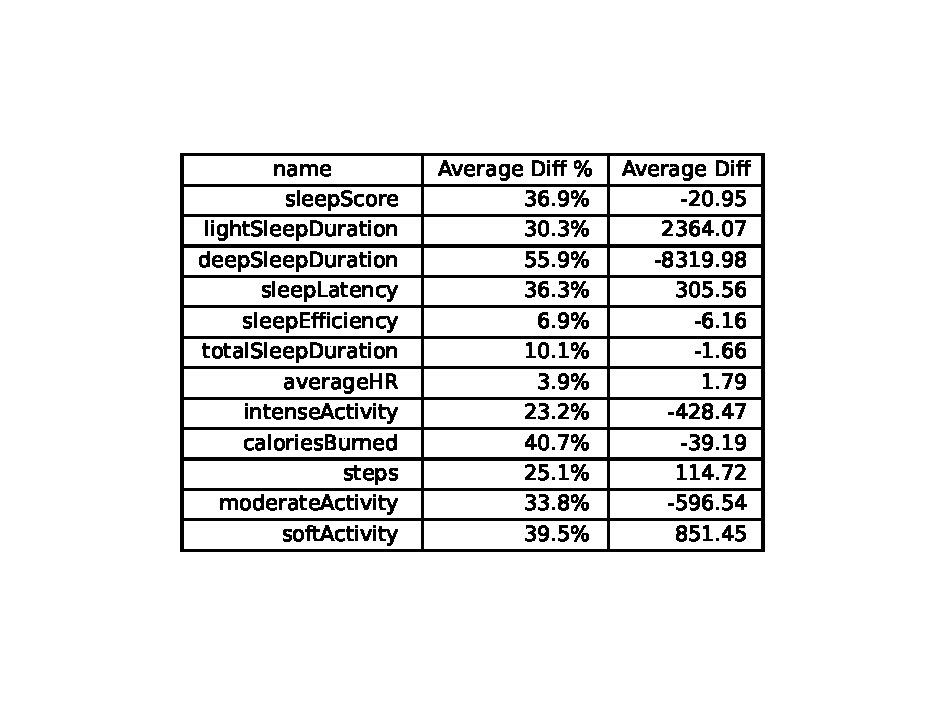
\includegraphics[width=\textwidth,keepaspectratio]{../images/empiricalResults.pdf}
    \caption{Empirical Differences Results}
    \label{fig:empirical}
    
\end{figure}

Two-tailed, Paired t-test was used to test this hypothesis. Student's t-test is preferred over Z-test because it does not require knowing the population variance, and it performs better with a smaller sample size. Paired version is used because measurements with different devices were taken from the same participant i.e. repeated measurement, which makes the measurements related. Also, equivalence bounds were calculated using TOST, which represents bounds of allowed tolerance, after which devices are equal; this is best shown via an example later on. Results: \ref{fig:results}.

\begin{figure}
    
    \centering
    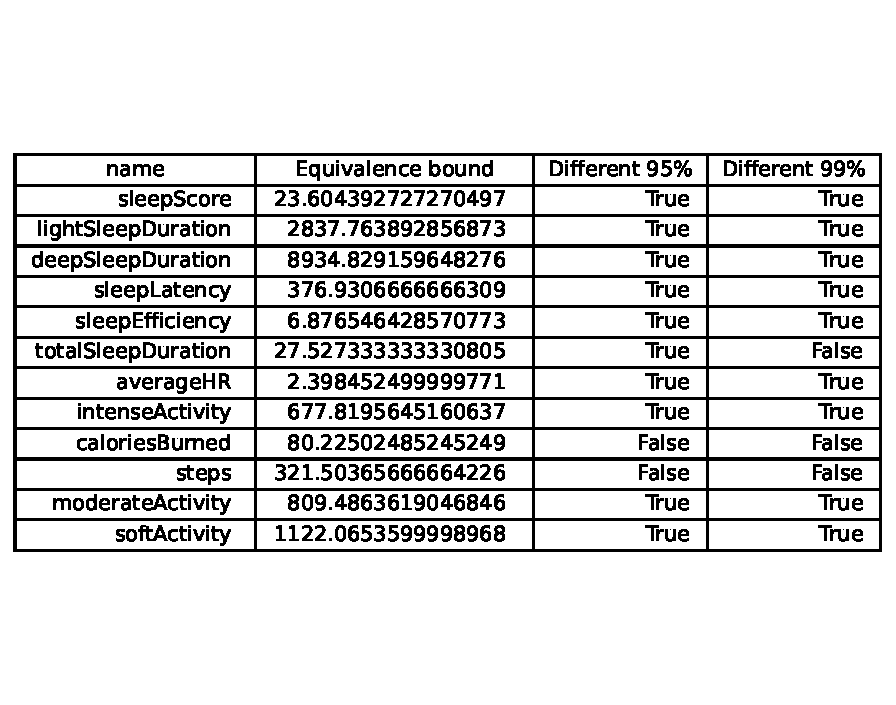
\includegraphics[width=\textwidth,keepaspectratio]{../images/results.pdf}
    \caption{Statistical Testing Results}
    \label{fig:results}
    
\end{figure}
\chapter{Evaluation}
\label{cha:evaluation}
\section{Comparing Devices}
\section{AI Response quality}
\section{Cost}


TODO: Do this chapter

\chapter{Conclusions}
\label{cha:evaluation}
\section{Summary of Achievements}
In summary, all project aims were fulfilled, except for the cost of service and ease of set-up aims. Other commercially available products cost less, while providing similar or better functions, and the service is very tough to self-deploy.

Core application - OpenFitCompanion was produced, an open-source alternative to health data aggregators and health companions. Providing convenient access to all data in one place with an option to export it to a file, enabling further research such as comparing health tracking devices. Employing nudging mechanisms via daily and weekly reports, where users can effortlessly examine: trends and progress towards their goals. Leveraging AI to create activity plans, curating exercises to align with user's preferences and needs, with exercise reminders sent via push-notifications. Lastly, enabling a natural language conversation about user's health data, mimicking interaction with a personal trainer at a fraction of the cost. System structure was explained with the help of diagrams and key decisions justified. If AI is not used, the application is a strong alternative to similar systems like Google Fit. Although, AI functions within the application can provide useful insights, it also raises the operating cost to where it is hard to justify that our product is a better alternative. 

Data analysis was performed in order to answer research question concerning the equivalence of used devices. Finding of exploration were presented: Bland-Altman plots, implications of initial findings and outlier protocol. Empirical difference percentages were calculated. Hypothesis testing problem was formulated, with the justification of statistical test used. Finally, results were interpreted showing evidence of significant difference in measurement of different activity intensity seconds. Still, it is merely an interesting observation that warrants conducting a more formal, rigorous study involving more participants and stricter data gathering methodology. The artefact could enable such studies to be performed in a cost-effective and transparent manner.
\section{Critical Reflection}
\subsection{Product \& Investigation}
Cost was one of the driving factors to develop OpenFitCompanion, so that users can enjoy features that commercial products lock behind a an expensive subscription. Although there is one product that OpenFitCompanion beats on cost, it loses to all others. Another model or approach should have been tried. 

Open-source was also a key point, however, a lot of closed source and non portable technologies have been used. Deploying on closed-source cloud like AWS and storing data in DynamoDB restrict options for further extension and possible migration. More open technologies should have been used to stay true to the product's name - OpenFitCompanion.

The project is not very attractive to potential open-source contributors due to absence of tests and a very manual deployment procedure. Tests allow collaborators to feel confident about system changes, ensuring no functional regression takes place. At least for very critical portions, tests should have been created. Regarding deployment process, the project requires zipping lambda function folders and uploading them on the AWS web console one by one after every change. For a project that is cloud-centric, more attention should have been dedicated to automating deployment pipeline.

User errors definitely took place during data collection for the analysis. They could caused differences between devices that were not detected via used outlier detection protocol. A more rigorous methodology for data collection should have been, such as journaling each day to sanity-check measurements from each device. 
\subsection{Personal}
I think the biggest difficulty was my lack of planning. As this project was self-proposed, I was in charge of coming up with requirements. Initially coming up with a very simplistic system that would not have enough complexity. My philosophy was to first finish that and if I have time then expand to more features. After finishing that simple application, with the help of my supervisor and wearables lab I got very interesting feature ideas  such as incorporating a second device and using LLMs. However, the foundation of the system was too simple and could not those features, so I have re-structured the system many times. I think I wasted a good chunk of time doing that, whereas I should have spent more time planning before implementation. Alternatively, I could have employed agile methodology and developed the system with high degrees of modularity and flexibility, therefore being able to cope with changing requirements more easily.

The previous point also lead to me not having a clear schedule, mostly bouncing between working on different features with no deadlines set. Especially with LLM integration, I spent too much time on designing prompts, trying to improve reliability, etc. This led me to have less time to polish other implementation aspects as well as working on the screencast and this report. I also tunnel-visioned on trying to make GPT4 work, whereas trying different models might have been more beneficial. 
\section{Further Work}
\subsection{Reducing AI inference cost}
\label{subsec:tryingOther}
As discussed in evaluation \ref{cha:evaluation}, the service does not compare well to other products mainly due to cost of using GPT4 with Knowledge Retrieval (RAG), which is still an experimental feature at the time of writing. Maybe OpenAI improves the feature and allows more tuning, however as it currently stands other models should be examined. An obvious choice would be open-source models like LLAMA-2 or recently released Grok-1, as on the surface they are free to use. However, they are hard to set up and require commercial level ML machines with a lot of VRAM, this is the reason they were not used initially. Cloud deployment is a more realistic prospect, with a rough estimate of using AWS Sagemaker to run LLAMA-2-13B on demand costing 7£ per month. Still, open-source models perform worse than commercial ones like GPT4, whether utility is preserved while reducing costs remains to be seen via experimentation.

The other option is to use newer commercial model. For example Claude 3 Sonnet, performs almost equally with GPT4, and even surpassing it, at a fraction of the cost. It is hard to classify which LLM benchmark reflects the nature of the task at hand, so the safe option is "Mixed evaluations (BIG-Bench-Hard)" benchmark, which contains a mix of different tasks, serving as a kind of an IQ test for LLMs. Sonnet has 82.9\% performance against 83.1\% of GPT4 \cite{claude3Bench}, while having a cost of 3\$ per 1M tokens, which is 333\% less than GPT4.

\subsection{Utilizing LLM vision}
First idea is to use visual modality in LLMs for nutrition management. Nutrition is as important as exercise or sleep for improving overall health. Existing commercial products mostly involve manually putting ingredients and it's quantity to estimate calories and macro-nutrients from the meal. However, this feature would involve just taking a picture of the meal, which is then processed by an LLM. MyfitnessPal has similar feature where you scan the meal using the camera; however, from the demo and user feedback, it is apparent that it requires having very cleanly separated ingredients which are scanned from different zoom levels separately, struggling with meals where ingredients are slightly mixed. Preliminary investigation using Claude 3 Sonnet shows promise, it guesses ingredients of a dish \ref{fig:sonnetV1} somewhat correctly, and then approximates the weight of each one \ref{fig:sonnetV2}.

Second idea is to force users to go to the gym by requiring taking a selfie in the gym on designated days. This would probably go beyond nudging and be considered an intervention. However, feeling that something is keeping you accountable can be encouraging as well. The process would involve taking a fresh picture of the user with some distinct gym equipment in the background, then using LLM to verify if its the same user and that they are in the gym. Camera API would be used rather than image upload, as users may upload old photos. Personalised encouraging messages could be sent on failure to verify, such as how many MET minutes the gym workout would contribute to reaching the weekly goal. 
\begin{figure}
    
    \centering
    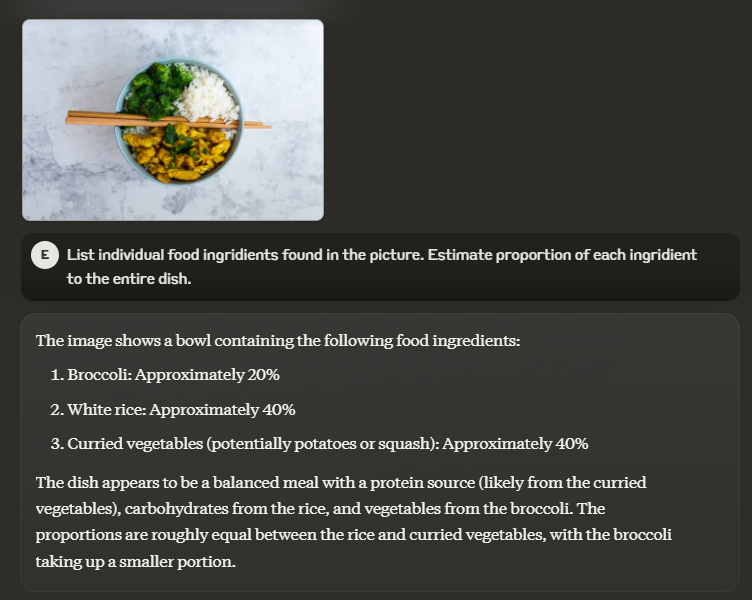
\includegraphics[width=1\textwidth,keepaspectratio]{../images/sonnet_vision.png}
    \caption{Claude 3 Sonnet identifies ingredients in a dish}
    \label{fig:sonnetV1}
    
\end{figure}
\begin{figure}
    
    \centering
    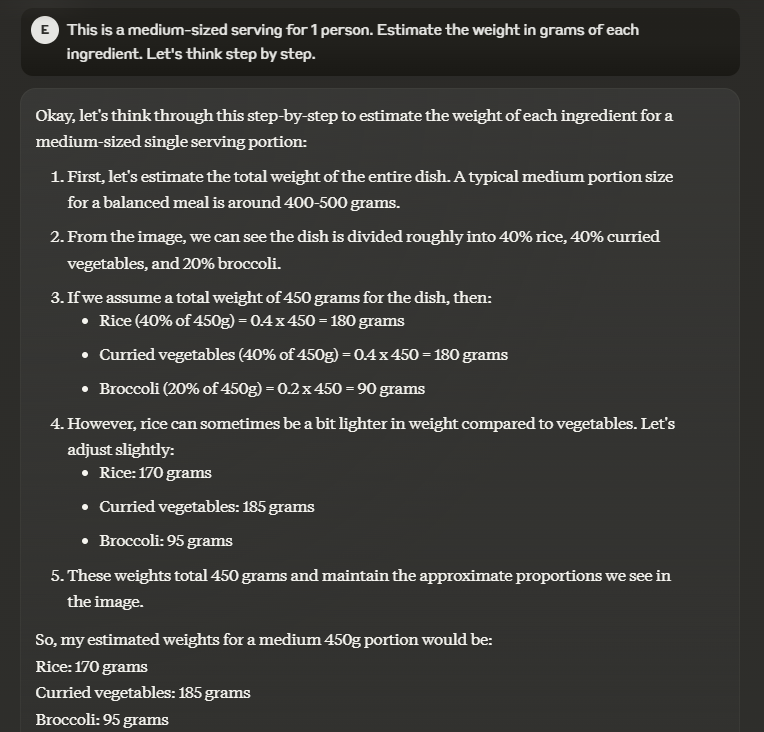
\includegraphics[width=1\textwidth,keepaspectratio]{../images/sonnet_vision_2.png}
    \caption{Claude 3 Sonnet approximates weight of each ingredient of a dish}
    \label{fig:sonnetV2}
    
\end{figure}

\subsection{Avoiding Cloud vendor lock-in}
Cloud providers like AWS try to make it hard to switch to another provider. For example, Lambda's data out is free of charge as long as the destination is another AWS service. AWS were to raise prices, it would be a laborious task to replicate the functionality on another cloud, like Azure. Then Azure could raise prices as well, requiring another rewrite or just accepting the situation and overpaying. 

One option is OpenStack. It is a fundamentally different approach - it is an open-source, private cloud solution. Whereby you have similar components of a typical cloud infrastructure but deployed on particular machine. OpenStack is software which can run on any linux machine, so it can be deployed on either a physical machine or a VM. Physical machine would involve maintenance, which would be unreasonable for most users. Deploying on a VM, like AWS EC2 instance would be more practical as it won't require physical maintenance. However, it would still involve a complex set-up. Taking this option woul make the project cloud provider independent, able to deploy on physical machines or on any VM from any provider. Notably, Mixtral provides ready to deploy OpenStack system to self-deploy their LLM, so this could tie with earlier suggestion \ref{subsec:tryingOther} of trying other LLM models 

Terraform is another option. It is an Infrastructure as Code (IAC) solution, allowing writing infrastructure using textual configuration files. CloudFormation is used within this project, but it only supports AWS only, whereas Terraform is cross-platform and supports all major cloud providers. It would not prevent lock-in like OpenStack would, but it would make it easier to migrate or use multi-cloud strategy. It would also improve existing self-deployment process, as it could automatically fill in template fields such as secret keys from a configuration file, whereas currently the user has to use web console and complete the process of filling variables manually.


  \bibliography{refs}    % this causes the references to be listed

\bibliographystyle{abbrv}
%% the bibliography style determines the format  in which both citations and references are printed,
%% other possible values are plain and abbrv
%%
%% If you want more control of the format of your citations you might want to take a look at
%% natbib.sty, which should be part of any standard LaTeX installation
%%
%% University regulations simply require that your citation style be consistent, so see what style
%% your supervisor recommends.


\end{document}
